\section{Action\-Random Class Reference}
\label{classActionRandom}\index{ActionRandom@{ActionRandom}}
Action, randomly generating monsters at specified map.  


{\tt \#include $<$actionrandom.hpp$>$}

Inheritance diagram for Action\-Random::\begin{figure}[H]
\begin{center}
\leavevmode
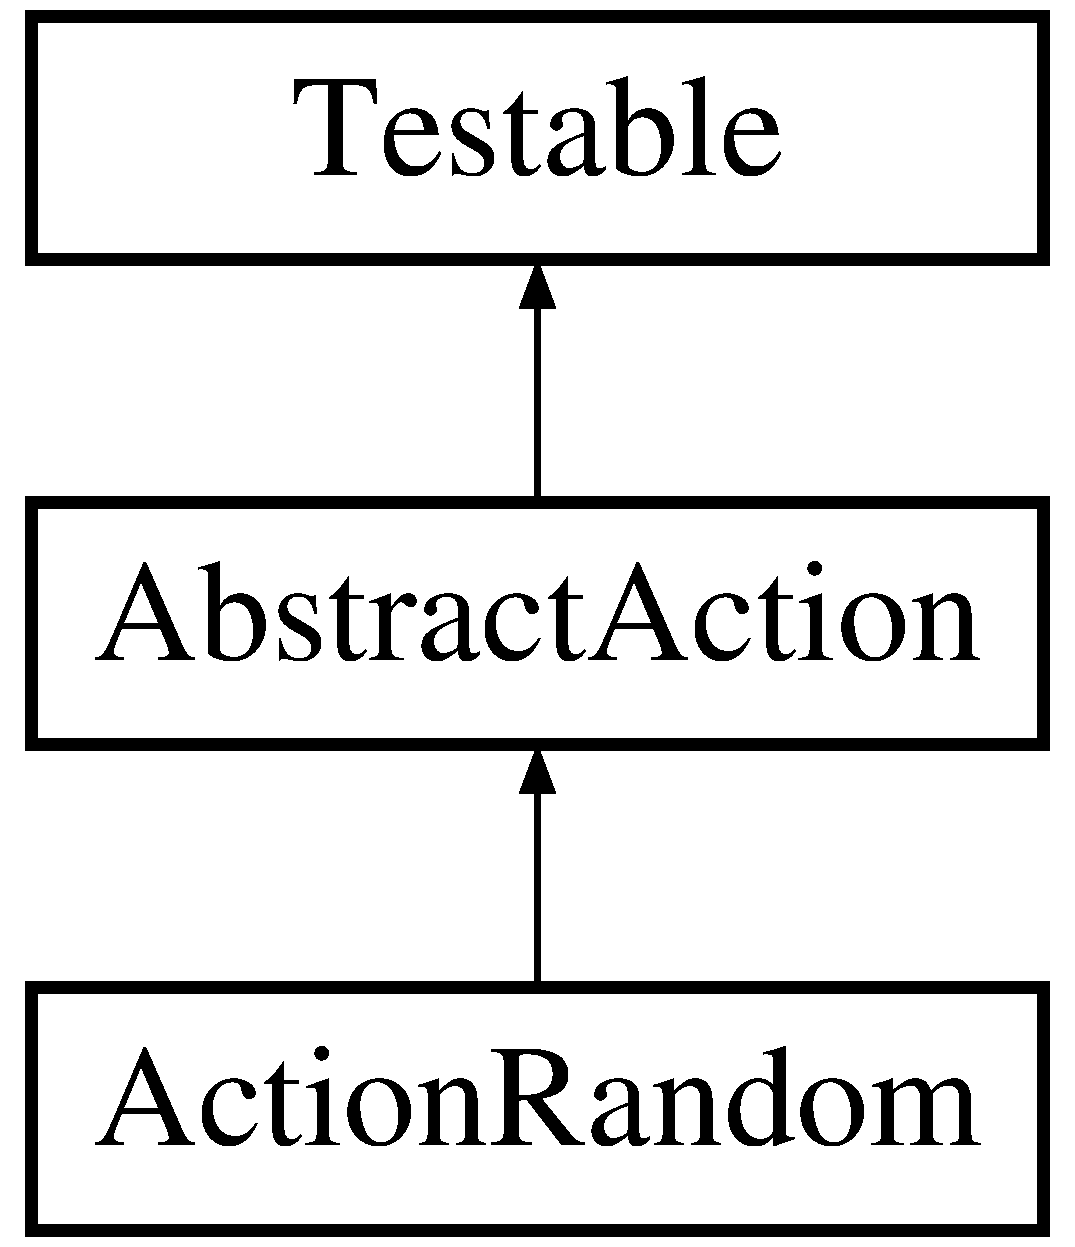
\includegraphics[height=3cm]{classActionRandom}
\end{center}
\end{figure}
\subsection*{Public Member Functions}
\begin{CompactItemize}
\item 
{\bf Action\-Random} ({\bf Parser} \&parser)
\item 
bool {\bf run} ({\bf Monster} \&\_\-monster)
\item 
void {\bf load} ({\bf Parser} \&parser)
\item 
void {\bf save} (ofstream \&file)
\item 
int {\bf test} (bool verbose) const 
\end{CompactItemize}
\subsection*{Protected Attributes}
\begin{CompactItemize}
\item 
int {\bf monsters\-Count}
\item 
{\bf Coordinates\-List} {\bf coordinates}
\item 
int {\bf monster\-Type}
\item 
QString {\bf map\-Name}
\end{CompactItemize}


\subsection{Detailed Description}
Action, randomly generating monsters at specified map. 



\subsection{Constructor \& Destructor Documentation}
\index{ActionRandom@{Action\-Random}!ActionRandom@{ActionRandom}}
\index{ActionRandom@{ActionRandom}!ActionRandom@{Action\-Random}}
\subsubsection{\setlength{\rightskip}{0pt plus 5cm}{\bf Action\-Random} ({\bf Parser} \& {\em parser})}\label{classActionRandom_a0}




\subsection{Member Function Documentation}
\index{ActionRandom@{Action\-Random}!load@{load}}
\index{load@{load}!ActionRandom@{Action\-Random}}
\subsubsection{\setlength{\rightskip}{0pt plus 5cm}void load ({\bf Parser} \& {\em parser})\hspace{0.3cm}{\tt  [virtual]}}\label{classActionRandom_a2}




Implements {\bf Abstract\-Action} {\rm (p.\,\pageref{classAbstractAction_a2})}.\index{ActionRandom@{Action\-Random}!run@{run}}
\index{run@{run}!ActionRandom@{Action\-Random}}
\subsubsection{\setlength{\rightskip}{0pt plus 5cm}bool run ({\bf Monster} \& {\em \_\-monster})\hspace{0.3cm}{\tt  [virtual]}}\label{classActionRandom_a1}




Implements {\bf Abstract\-Action} {\rm (p.\,\pageref{classAbstractAction_a1})}.\index{ActionRandom@{Action\-Random}!save@{save}}
\index{save@{save}!ActionRandom@{Action\-Random}}
\subsubsection{\setlength{\rightskip}{0pt plus 5cm}void save (ofstream \& {\em file})\hspace{0.3cm}{\tt  [virtual]}}\label{classActionRandom_a3}




Implements {\bf Abstract\-Action} {\rm (p.\,\pageref{classAbstractAction_a3})}.\index{ActionRandom@{Action\-Random}!test@{test}}
\index{test@{test}!ActionRandom@{Action\-Random}}
\subsubsection{\setlength{\rightskip}{0pt plus 5cm}int test (bool {\em verbose}) const\hspace{0.3cm}{\tt  [virtual]}}\label{classActionRandom_a4}




Implements {\bf Testable} {\rm (p.\,\pageref{classTestable_a0})}.

\subsection{Member Data Documentation}
\index{ActionRandom@{Action\-Random}!coordinates@{coordinates}}
\index{coordinates@{coordinates}!ActionRandom@{Action\-Random}}
\subsubsection{\setlength{\rightskip}{0pt plus 5cm}{\bf Coordinates\-List} {\bf coordinates}\hspace{0.3cm}{\tt  [protected]}}\label{classActionRandom_p1}


\index{ActionRandom@{Action\-Random}!mapName@{mapName}}
\index{mapName@{mapName}!ActionRandom@{Action\-Random}}
\subsubsection{\setlength{\rightskip}{0pt plus 5cm}QString {\bf map\-Name}\hspace{0.3cm}{\tt  [protected]}}\label{classActionRandom_p3}


\index{ActionRandom@{Action\-Random}!monstersCount@{monstersCount}}
\index{monstersCount@{monstersCount}!ActionRandom@{Action\-Random}}
\subsubsection{\setlength{\rightskip}{0pt plus 5cm}int {\bf monsters\-Count}\hspace{0.3cm}{\tt  [protected]}}\label{classActionRandom_p0}


\index{ActionRandom@{Action\-Random}!monsterType@{monsterType}}
\index{monsterType@{monsterType}!ActionRandom@{Action\-Random}}
\subsubsection{\setlength{\rightskip}{0pt plus 5cm}int {\bf monster\-Type}\hspace{0.3cm}{\tt  [protected]}}\label{classActionRandom_p2}




The documentation for this class was generated from the following files:\begin{CompactItemize}
\item 
{\bf actionrandom.hpp}\item 
{\bf actionrandom.cpp}\end{CompactItemize}
